\chapter{Results}\label{chap:results}
\begin{chapabstract}

In this chapter, I present our results with figures.
Firstly, in Section~\ref{sec:GammaDistribution}, I show the $\qn$ frequency dependence for each galaxy with the distribution of $\gamma$.
Secondly, in Section~\ref{sec:sfrfromlowradio}, I show the result of the comparison between the SFR from a radio emission and other indicators.

\end{chapabstract}


%\section{Final samples}
%
%Here, I will mention 18 samples and put the figure to compare it with CalistroRivera2017a.

\section{Distributions of $\gamma$}\label{sec:GammaDistribution}

\begin{figure}[htbp]
	\centering
	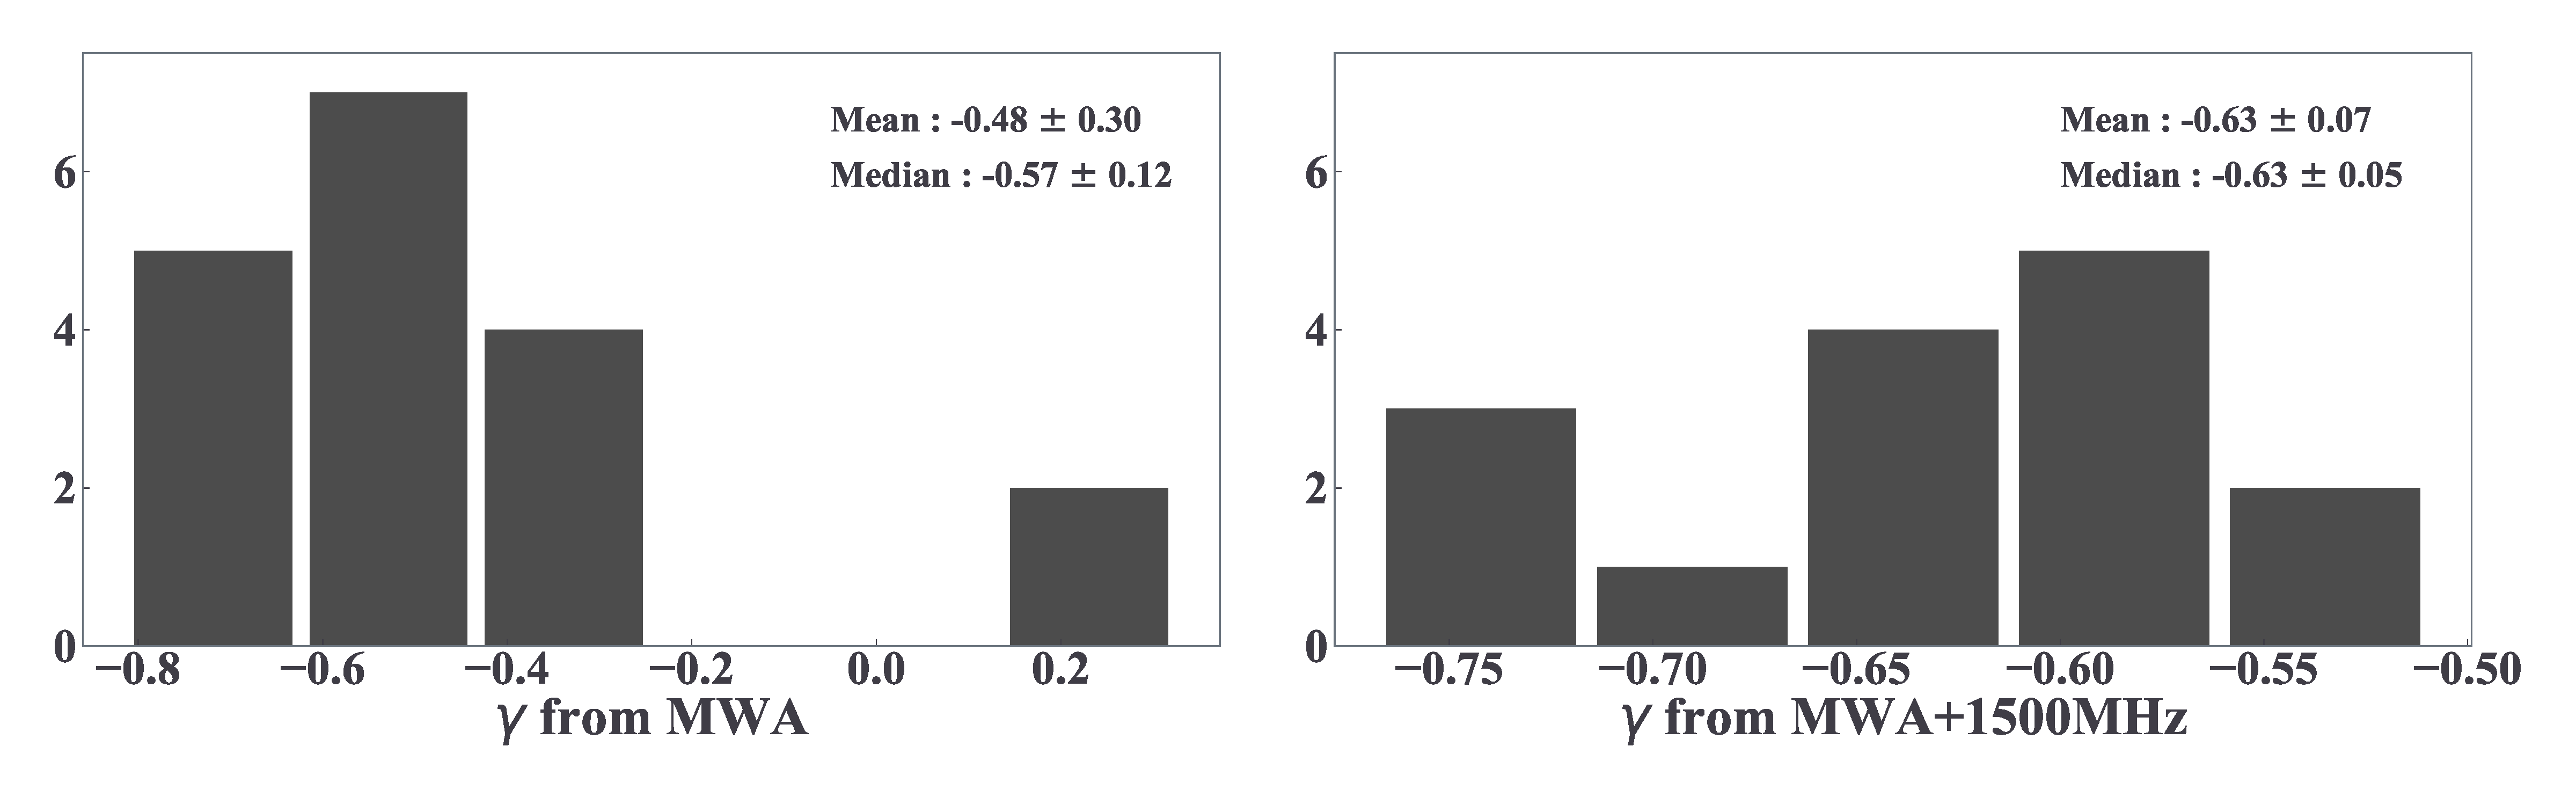
\includegraphics[width=\linewidth]{Chapter_5/Figures/Result_comparehist.pdf}
    \caption[Histograms of $\gamma$ from the fitting]{\label{fig:comparehist}
        This figure shows distributions of $\gamma$ for each fitting.
        The left figure indicates the fitting result with only MWA frequencies, and the right one does with 1500 [MHz] besides MWA frequencies.
    }
\end{figure}

\begin{figure}[htbp]
	\centering
	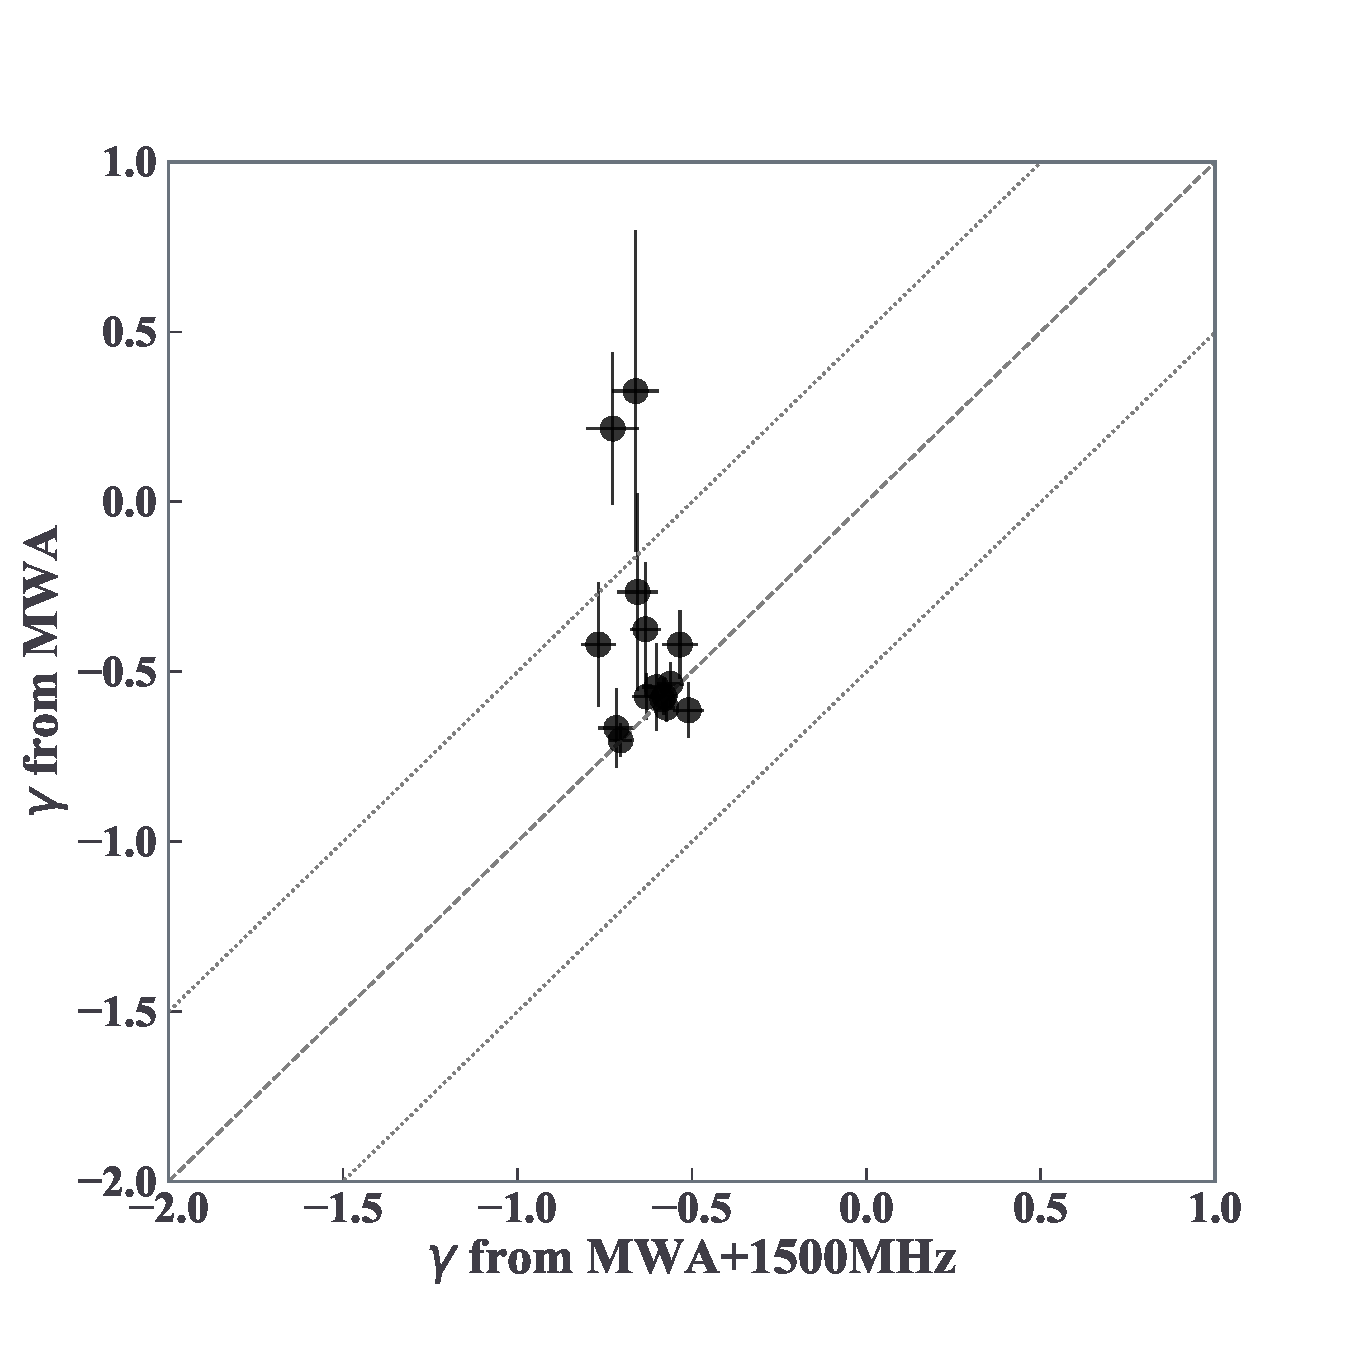
\includegraphics[width=.6\linewidth]{Chapter_5/Figures/Result_comparealpha.pdf}
    \caption[The comparison of $\gamma$ from different fitting methods]{\label{fig:comparegamma}
        This figure is for comparing the difference of $\gamma$ for each fitting method.
        The solid line shows the one to one correlation, and dotted lines show 0.5 dex away from the solid line.
        Each plot shows each galaxy.
        In this figure, we can see $\gamma$ fitted to only MWA frequencies are relatively flatter.
    }
\end{figure}

Here, we show two kinds of fitting results.
The left plot in Figure~\ref{fig:comparehist} is the $\gamma$ distribution from the fitting only to MWA frequencies, and the right one is to $1500\MHz$ besides MWA frequencies.
We show the mean and median with the standard and quantile deviation in both plots.
Since we adopt high-quality flux data at $1500\MHz$ \citep{Boselli2015}, three samples (HRS 122, 163 and 204) are fitted only in the case with MWA fluxes.
Figure~\ref{fig:comparegamma} compares $\gamma$ from different fitting fluxes for each galaxy.

In these figures, we can find that there are two galaxies (HRS 25 and 144) with a relatively flatter $\gamma$ fitted only to MWA frequencies.
This suggests that there is a critical frequency where the turnover arises between MWA frequencies and $1500\MHz$.
At low frequencies, the spectral is prone to be flatter due to the free-free absorption \citep[e.g.,][]{CalistroRivera2017a, Schober2017, Chyzy2018}.
In addition to this, \citet{Schober2017} show that a Milky Way like galaxy (similar SFR) has the critical frequency order of magnitude lower than the MWA frequency.
However, HRS 25 and 144 have a Milky Way like SFR \citep{Boselli2015} and a critical frequency between MWA frequencies and $1500\MHz$.
This result cannot be explained by \citet{Schober2017}.
One possible explanation is that fewer number of fluxes yields less constraint of the fitting and the flatter $\gamma$ for HRS 25 and the galactic nuclei affects the spectral for HRS 144 identified as a Seyfert galaxy from the BPT diagram \citep[e.g.,][]{Baldwin1981, Kewley2001, Kauffmann2003, Schawinski2007}.
For understanding these galaxies, we would need the case study with more data in a wide frequency range.

If we neglect these galaxies, the mean $\gamma$ changes from $-0.48\pm0.30$ to $-0.57\pm0.14$ for the fitting without $1500\MHz$ and from $-0.63\pm0.08$ to $-0.62\pm0.08$ with $1500\MHz$.
The mean $\gamma$ does not vary in any case with $1500\MHz$.
This means that HRS 25 and 144 do not affect the fitting result among MWA frequencies and $1500\MHz$, although they do the mean $\gamma$ from the fitting only to MWA frequencies.
Therefore, in this paper, we adopt the averaged $\gamma$ obtained from the fitting across the MWA frequency to $1500\MHz$ for calculating SFR (Section~\ref{sec:sfrfromlowradio}).\\
The fitting results are shown in Appendix~\ref{chap:fittingresults}.



\section{Comparing SFR indicators}\label{sec:sfrfromlowradio}

\begin{figure}[htbp]
	\centering
	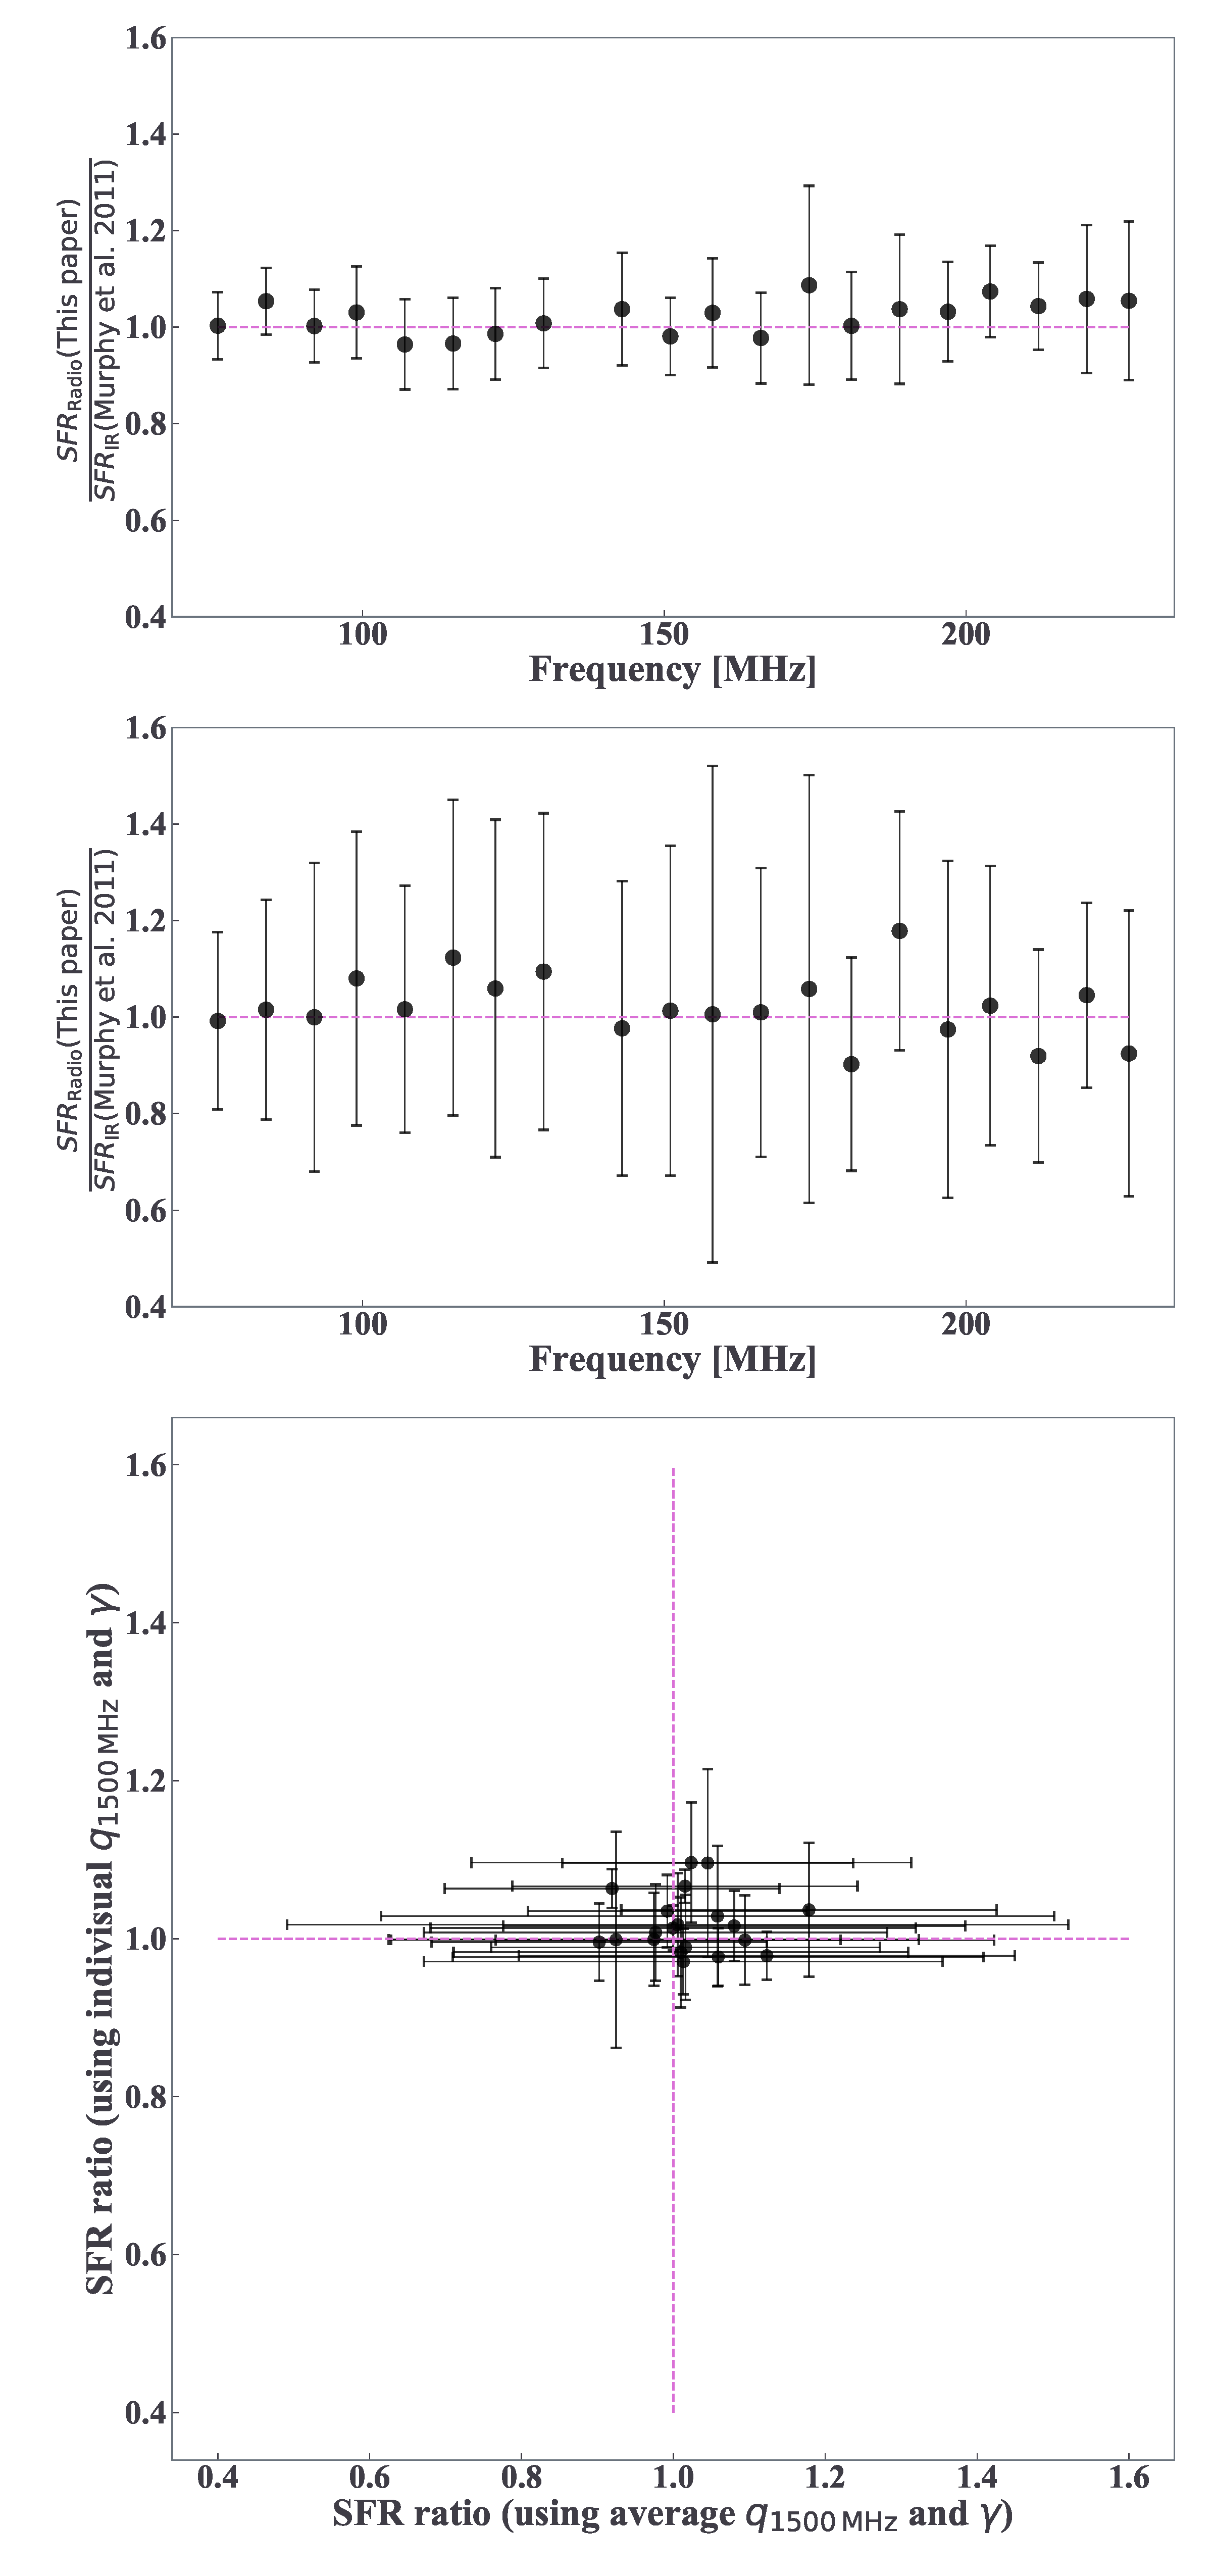
\includegraphics[width=.6\linewidth]{Chapter_5/Figures/Result_sfrratio.pdf}
    \caption[The consistency of the radio SFR]{\label{fig:sfrratio}
        This figure shows the SFR ratio between $\mr{SFR}_{\mr{Radio},\,\nu}$ and $\mr{SFR}\msb{IR}$ at each MWA frequency.
        The difference between the upper and middle plots is the calibration parameters to calculate $\mr{SFR}_{\mr{Radio},\,\nu}$.
        Individual or averaged $\gamma$ and $\q{1500\MHz}$ are used for the upper or middle plots, respectively.
    The bottom plot compares SFR ratios calculated with different calibrations.
    }
\end{figure}

\begin{figure}[htbp]
	\centering
	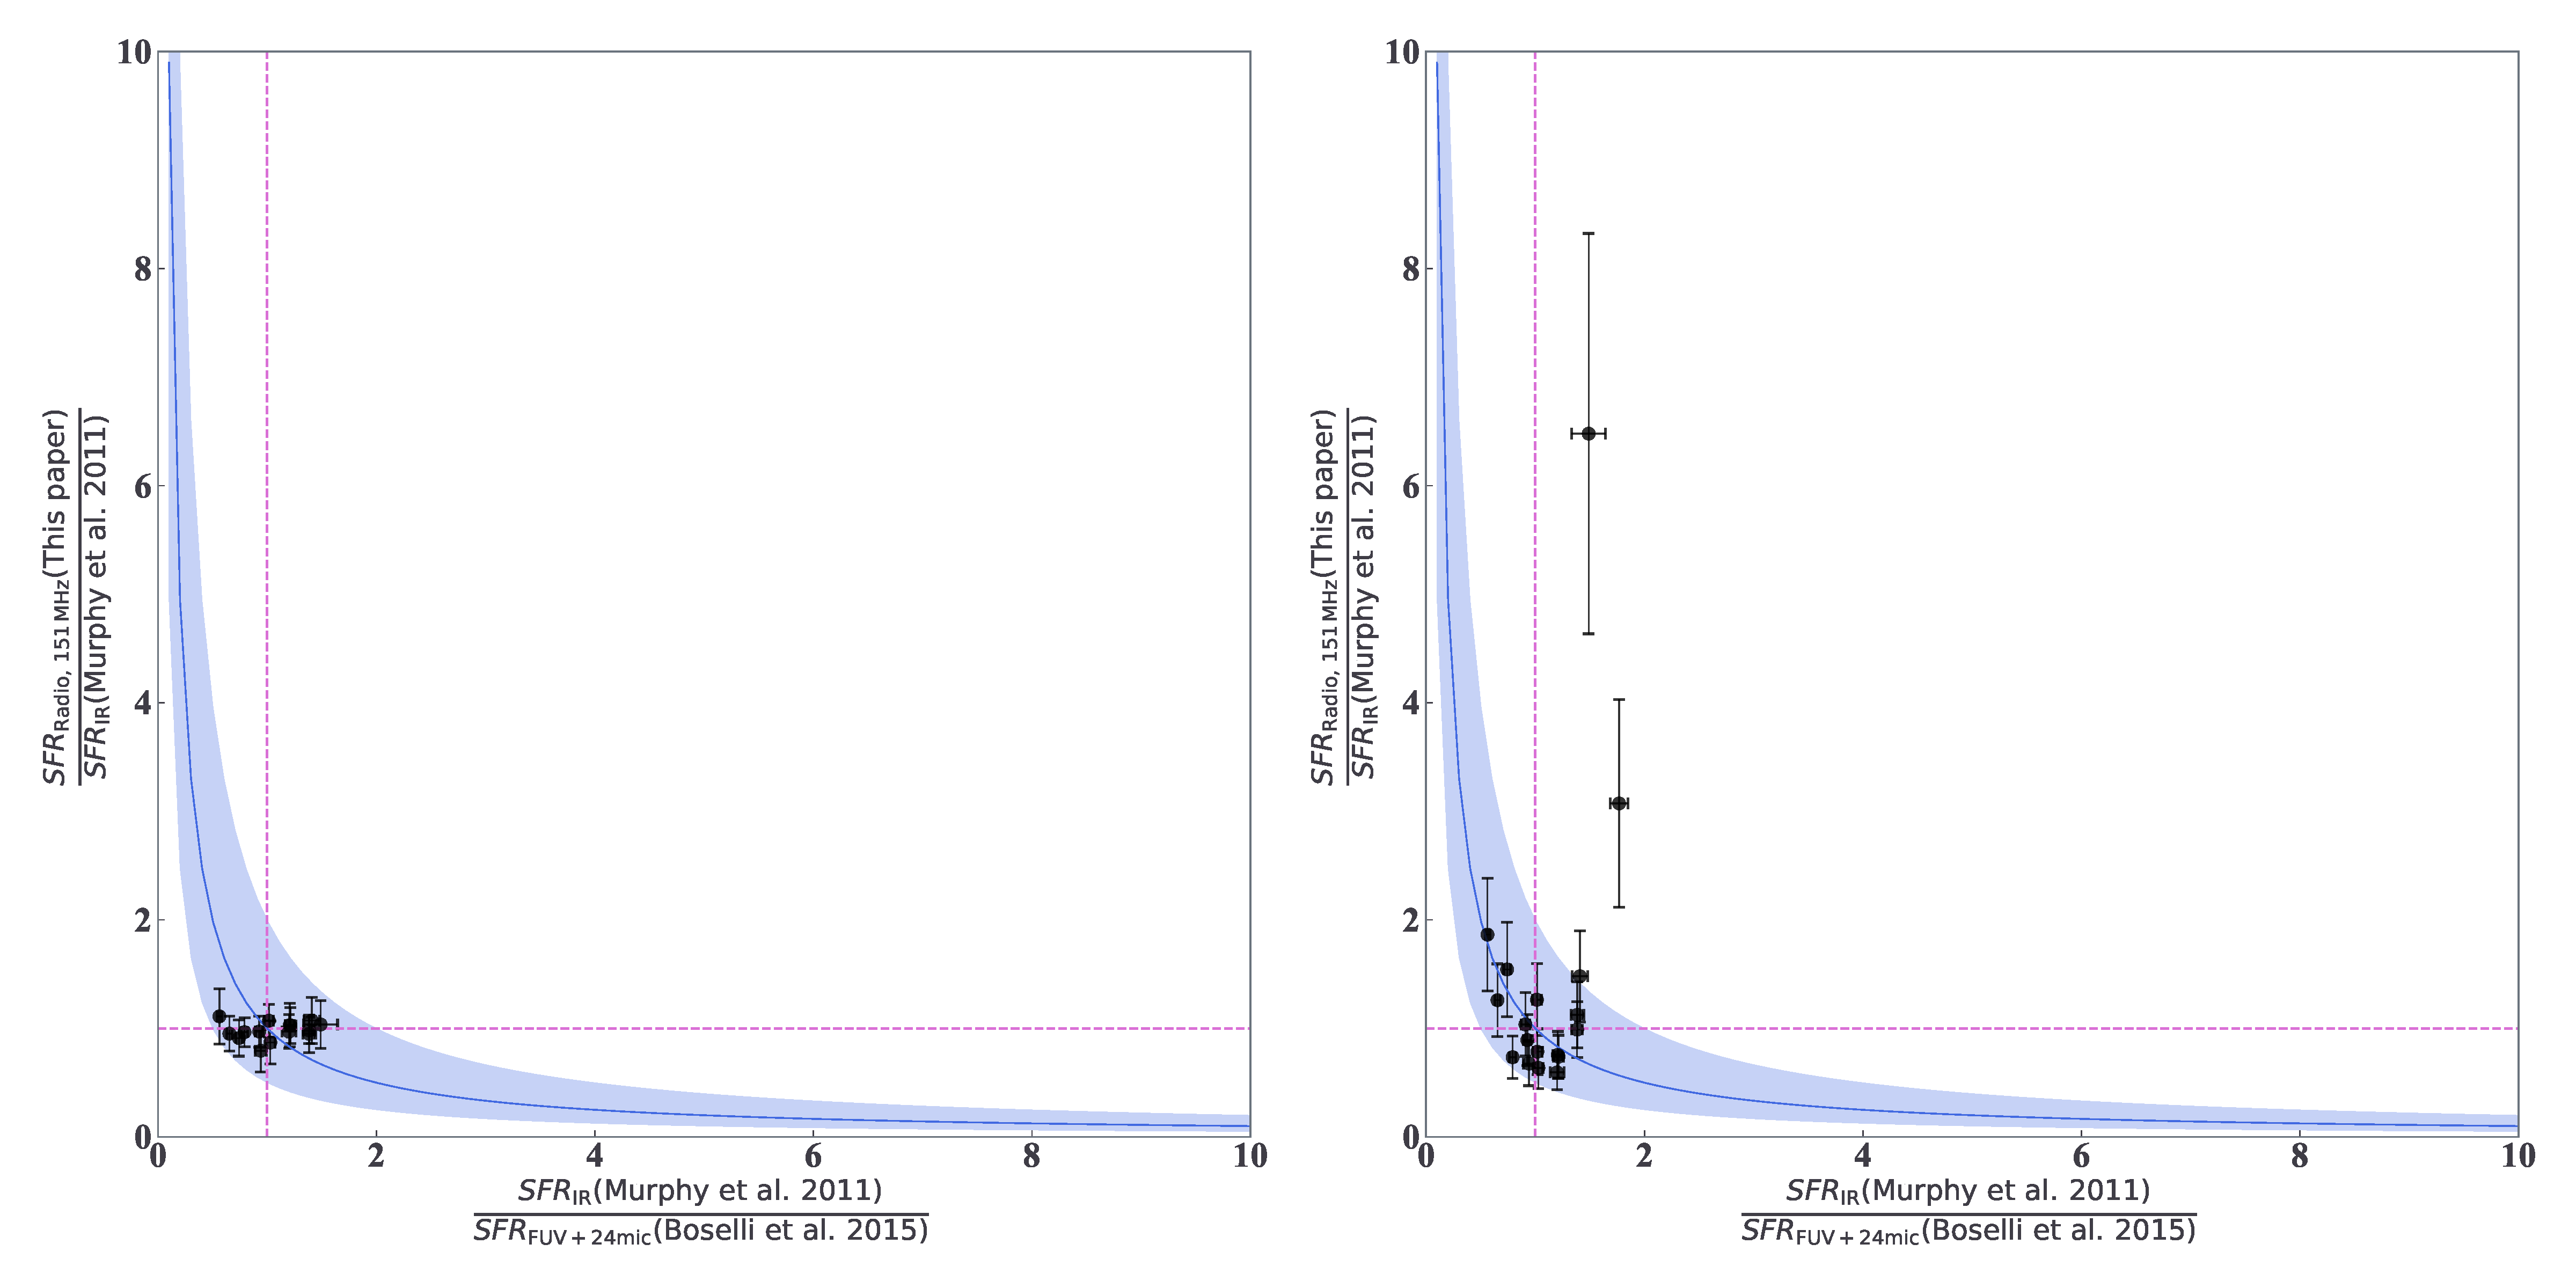
\includegraphics[width=\linewidth]{Chapter_5/Figures/Result_sfrratios.pdf}
    \caption[The consistency of the radio SFR with $\mr{SFR}\msb{IR}$ and $\mr{SFR}\msb{FUV+24mic}$]{\label{fig:sfrratios}
        This figure shows SFR ratios from different indicators.
        The vertical and horizontal axes are $\mr{SFR}\msb{Radio,\,151\MHz}\ /\ \mr{SFR}\msb{IR}$ and $\mr{SFR}\msb{IR}\ /\ \mr{SFR}\msb{FUV+24mic}$ in both plots.
        Magenta dashed lines indicate the unity for each SFR ratio, and the solid blue lines do for the SFR ratio between $\mr{SFR}\msb{Radio,\,151\MHz}\ /\ \mr{SFR}\msb{FUV+24mic}$.
        The blue shaded region shows the ratio between $\mr{SFR}_{\mr{Radio},\,151\MHz}$ and $\mr{SFR}\msb{FUV+24mic}$ within factor two ($0.5 \leq \mr{SFR}_{\mr{Radio},\,151\MHz}\ /\ \mr{SFR}\msb{FUV+24mic} \leq 2$).
        The difference between the upper and middle plots is the calibration parameters to calculate $\mr{SFR}_{\mr{Radio},\,151\MHz}$.
    }
\end{figure}

Here, we show the result from comparing $\mr{SFR}_{\mr{Radio},\,\nu}$ defined by Equation~\ref{eq:sfrfromradio} with $\mr{SFR}\msb{IR}$ (Equation~\ref{eq:sfrir}) and $\mr{SFR}\msb{FUV+24mic}$ \citep{Boselli2015}.

Figure~\ref{fig:sfrratio} shows the SFR ratio between $\mr{SFR}_{\mr{Radio},\,\nu}$ and $\mr{SFR}\msb{IR}$.
For drawing the upper figure, we substitute the individual $q_{1500\MHz}$ and $\gamma$ into Equation~\ref{eq:sfrfromradio}.
We calculate $\mr{SFR}_{\mr{Radio},\,\nu}$ at each MWA frequency and plot the mean value.
Note that the number of galaxies taken for the mean at each frequency is different because we use only high-quality fluxes.
In this case, we can see it is consistent with $\mr{SFR}\msb{IR}$ within a 10\% error.
For the middle figure, we substitute the averaged $q_{1500\MHz}$ and $\gamma$ instead of individual values.
This calibration method yields larger scatters compared to the previous one.
However, $\mr{SFR}_{\mr{Radio},\,\nu}$ is still consistent with $\mr{SFR}\msb{IR}$.
The bottom figure shows the SFR ratio comparison from different calibrations.
In this figure, it is clear that SFR calculated from the averaged value has more extensive scatters than from the individual values.

These figures give us the idea that calculating radio SFR needs the spectral energy distribution for less uncertainty.
For the spectral, we find that the single power-law assumption yields the radio SFR with the consistency within 10\%, even including galaxies that might have a flatter spectral at low frequencies.

Figure~\ref{fig:sfrratios} shows the comparison of SFR ratios.
For both plots in the figure, vertical and horizontal axes show the ratio between $\mr{SFR}_{\mr{Radio},\,151\MHz}$ and $\mr{SFR}\msb{IR}$, between $\mr{SFR}\msb{IR}$ and $\mr{SFR}\msb{FUV+24mic}$, respectively.
We use radio emission at $151\MHz$ because this is the only flux band that all our samples have high-quality data.
Here, we check the consistency of the radio SFR with other SFR indicators.
While $\mr{SFR}\msb{IR}$ traces the only dust emission, $\mr{SFR}\msb{FUV+24mic}$ does the direct young massive stellar emission dust-corrected with the radiation at $24\,\micron$ \citep{Murphy2011, Kennicutt2012}.
This figure shows how consistent the radio SFR is with this direct emission tracer.
The difference between these plots is the calibration parameter for calculating $\mr{SFR}_{\mr{Radio},\,151\MHz}$.
The individual $q_{1500\MHz}$ and $\gamma$ are used for the left plot and the averaged ones for the right plot.
The blue shaded region shows the ratio between $\mr{SFR}_{\mr{Radio},\,151\MHz}$ and $\mr{SFR}\msb{FUV+24mic}$ within factor two ($0.5 \leq \mr{SFR}_{\mr{Radio},\,151\MHz}\ /\ \mr{SFR}\msb{FUV+24mic} \leq 2$).
In the figure, we can see that the radio SFR using individual parameters is also consistent with $\mr{SFR}\msb{FUV+24mic}$.
However, in the other case, there are two galaxies (HRS 306 and 144) whose radio SFR overestimates.
This is because these galaxies have stronger radio emission (lower $\qn$) than the extrapolated average value at $151\MHz$.



%\bibliographystyle{mnras}
%%\bibliography{example} % if your bibtex file is called example.bib
%\bibliography{masterthesis}
